\documentclass[pdflatex,sn-basic]{sn-jnl}

% ---------------------------------------------------------------------------
% Empirical Software Engineering (Springer) build.
%
% Same sections, same generated numbers, same analysis as the IEEEtran build in
% ../main.tex. Only the frame differs: Springer's single column, EMSE's
% single-blind review (so the authors are named), and the declarations the
% journal requires.
%
% Figures are redrawn at Springer's 372pt text width rather than scaled up from
% the IEEE column:
%   MCP_FIG_DIR=paper/emse/figures MCP_FIG_WIDTH_IN=5.147 \
%   MCP_FIG_FONT_SCALE=1.1 python driver/make_figures.py
%
% Numeric macros are AUTO-GENERATED -- never hand-edit them; edit the analysis.
% ---------------------------------------------------------------------------

\usepackage{newtxtext,newtxmath}  % Times body, so the figures and the text
                                 % share a typeface
\usepackage{booktabs}
\usepackage{graphicx}
\usepackage{xcolor}
\usepackage{listings}
\usepackage{amsmath}
\usepackage{url}
\usepackage{hyperref}

\graphicspath{{figures/}}
% The sections were written against a numeric style, so every \\cite sits
% where a bracketed reference would. Under author-year it has to read as a
% parenthetical rather than as the subject of the sentence.
\let\cite\citep
% The shared sections input tables by a path relative to ../, so let LaTeX
% look there as well as here.
\makeatletter\def\input@path{{../}{./}}\makeatother

% AUTO-GENERATED by driver/make_numbers.py -- do not edit by hand.
\newcommand{\Nframe}{17,432}
\newcommand{\Nattempted}{6,106}
\newcommand{\NHarnessError}{17}
\newcommand{\NHarnessErrorPct}{0.3\%}
\newcommand{\NWithheld}{321}
\newcommand{\NDisclosureHigh}{146}
\newcommand{\NKilled}{32}
\newcommand{\NKilledPct}{0.5\%}
\newcommand{\NInterrupted}{49}
\newcommand{\NInterruptedPct}{0.8\%}
\newcommand{\NInterruptedNoHandshake}{48}
\newcommand{\NInterruptedDepressionPP}{0.8}
\newcommand{\Nprobed}{6,089}
\newcommand{\NNeedsConfig}{299}
\newcommand{\NMalformedOpaque}{8}
\newcommand{\NMalformedGo}{5}
\newcommand{\NEntrypointSeen}{466}
\newcommand{\NEntrypointUnreprobed}{4}
\newcommand{\HandshakeRateCl}{60.5\% (95\% CI 56.2--64.0)}
\newcommand{\ErrAsResultRateCl}{88.4\% (95\% CI 86.6--90.0)}
\newcommand{\NoTypecheckRateCl}{7.4\% (95\% CI 5.9--9.2)}
\newcommand{\MalformedDiesRateCl}{0.5\% (95\% CI 0.3--0.7)}
\newcommand{\GapRunnableCl}{16.1 pp (95\% CI 7.2--23.9)}
\newcommand{\GapErrAsResultCl}{-2.5 pp (95\% CI -6.0--1.6)}
\newcommand{\PctVerOffered}{97\%}
\newcommand{\NVerOffered}{3,576}
\newcommand{\NVerDowngraded}{104}
\newcommand{\NVerAhead}{5}
\newcommand{\TopPublisherHandshake}{26.2\%}
\newcommand{\TopPublisherDepressionPP}{1.8}
\newcommand{\HandshakeDesignEffect}{3.2}
\newcommand{\Nresponders}{3,685}
\newcommand{\HandshakeRate}{60.5\% (95\% CI 59.3--61.7)}
\newcommand{\HandshakeCount}{3685}
\newcommand{\ErrAsResultRate}{88.4\% (95\% CI 87.3--89.4)}
\newcommand{\ErrAsResultCount}{3,258}
\newcommand{\NotErrAsResultPct}{11.6\%}
\newcommand{\UnknownProtoErrCount}{139}
\newcommand{\UnknownWrongCodeCount}{122}
\newcommand{\UnknownProseCount}{166}
\newcommand{\NoTypecheckRate}{7.4\% (95\% CI 6.6--8.3)}
\newcommand{\MalformedDiesRate}{0.5\% (95\% CI 0.3--0.7)}
\newcommand{\SilentExecTS}{114}
\newcommand{\SilentExecPy}{0}
\newcommand{\SilentExecTSvOne}{108}
\newcommand{\SilentExecTSCaret}{111}
\newcommand{\SilentExecTSExact}{0}
\newcommand{\SDKPopTS}{2,449}
\newcommand{\SDKPopPy}{1,027}
\newcommand{\SDKIndirect}{100}
\newcommand{\SDKDirect}{3,385}
\newcommand{\SDKUnattributed}{200}
\newcommand{\SDKNoSDK}{182}
\newcommand{\SDKNoSDKRate}{47\%}
\newcommand{\Npublishers}{3,899}
\newcommand{\NuniqPub}{3,899}
\newcommand{\TopPublisherN}{305}
\newcommand{\TopPublisherPct}{5.0\%}
\newcommand{\TopTenPct}{12.6\%}
\newcommand{\HandshakeRatePub}{58.7\% (95\% CI 57.2--60.2)}
\newcommand{\ErrAsResultRatePub}{85.2\% (95\% CI 83.7--86.6)}
\newcommand{\NoTypecheckRatePub}{8.1\% (95\% CI 7.0--9.3)}
\newcommand{\NEntrypointBlocked}{462}
\newcommand{\EntrypointBlockedPct}{21.6\%}
\newcommand{\EntrypointRecovered}{44}
\newcommand{\EntrypointRecoveryRate}{9.5\% (95\% CI 7.2--12.5)}
\newcommand{\HandshakeCountCorr}{3,729}
\newcommand{\HandshakeRateCorr}{61.2\% (95\% CI 57.7--64.4)}
\newcommand{\HandshakeRateCorrBinom}{61.2\% (95\% CI 60.0--62.5)}
\newcommand{\NpmRate}{66.2\%}
\newcommand{\NpmN}{3,952}
\newcommand{\PypiN}{2,137}
\newcommand{\PypiRateRaw}{50.1\%}
\newcommand{\PypiRateCorr}{52.1\% (95\% CI 46.3--59.1)}
\newcommand{\GapRaw}{16.1}
\newcommand{\GapCorr}{14.0}
\newcommand{\NAcceptInvalid}{273}
\newcommand{\NSilentExec}{129}
\newcommand{\SilentExecShare}{47\%}
\newcommand{\SilentExecRate}{3.5\% (95\% CI 3.0--4.1)}
\newcommand{\NInBandError}{118}
\newcommand{\InBandShare}{43\%}
\newcommand{\NUnclassifiable}{26}
              % \Nframe, \Neligible, \Nprobed, ... (generated)
% AUTO-GENERATED by validation/make_validation_numbers.py.
\newcommand{\ValN}{40}
\newcommand{\ValAgree}{34}
\newcommand{\ValKappa}{0.70}
\newcommand{\ValPrecision}{95\%}
\newcommand{\ValRecall}{78\%}
\newcommand{\ValSilN}{19}
\newcommand{\ValInbN}{21}
\newcommand{\ValSilExecPct}{95\%}
\newcommand{\ValInbExecPct}{24\%}
\newcommand{\NSilentExecCorrected}{150}
\newcommand{\NSilentExecCorrectedLo}{110}
\newcommand{\NSilentExecCorrectedHi}{181}
   % \ValKappa, \ValPrecision, ... (generated)
\newcommand{\theauthor}{the author}
% AUTO-GENERATED by driver/compare_runs.py -- do not edit by hand.
% July census against the September re-run of the same frame.
\newcommand{\SeptDate}{26 September 2026}
\newcommand{\SDKTwoDate}{28 July 2026}
\newcommand{\NSeptGraded}{6,097}
\newcommand{\NSeptHandshake}{3,140}
\newcommand{\SeptHandshakeRate}{51.5\%}
\newcommand{\NRerunCommon}{6,106}
\newcommand{\NLost}{617}
\newcommand{\NGained}{72}
\newcommand{\NLostUnchanged}{615}
\newcommand{\NSDKTwoBroke}{564}
\newcommand{\NSDKTwoRange}{548}
\newcommand{\NpmWas}{2,615}
\newcommand{\NpmLost}{17}
\newcommand{\NpmLostRate}{0.7\%}
\newcommand{\PypiWas}{1,070}
\newcommand{\PypiLost}{600}
\newcommand{\PypiLostRate}{56.1\%}
\newcommand{\NPySDKWas}{1,027}
\newcommand{\NPySDKNow}{435}
\newcommand{\PySDKLostRate}{58\%}
\newcommand{\SeptErrAsResult}{88.2\%}
\newcommand{\SeptNoTypecheck}{9.0\%}
\newcommand{\SeptMalformedDies}{0.6\%}
\newcommand{\NPaired}{3,068}
\newcommand{\PairedEarBefore}{88.6\%}
\newcommand{\PairedEarAfter}{88.6\%}
\newcommand{\PairedTypeBefore}{8.8\%}
\newcommand{\PairedTypeAfter}{8.7\%}
\newcommand{\PairedMalBefore}{0.5\%}
\newcommand{\PairedMalAfter}{0.5\%}
\newcommand{\LostTypeRate}{0.3\%}
\newcommand{\PoisonOptionalPct}{29\%}
\newcommand{\NPinTested}{12}
\newcommand{\NPinRestored}{12}
\newcommand{\PySDKLostCI}{58\% (95\% CI 55--61)}
 % July against the September re-run (generated)
% Generated by driver/check_disclosure_status.py -- do not hand-edit.
% Maintainer response to the disclosure log, read back from GitHub.
% Last checked: 2026-09-26
\newcommand{\NMalformedDies}{17}
\newcommand{\NMalformedReported}{15}
\newcommand{\NMalformedUnreachable}{2}
\newcommand{\NMalformedFixed}{6}
\newcommand{\NMalformedReleased}{5}
\newcommand{\NSilentNotices}{129}
   % \NMalformedFixed, ... (generated)

% EMSE reviews single-blind, so this build carries the real artifact location.
\newcommand{\ArtifactURL}{\url{https://github.com/Ahmad-Faraj/mcp-conformance}}

\begin{document}

\title[An Execution-Based Conformance Census of the MCP Registry]{Installed,
Launched, Probed: An Execution-Based Conformance Census of the Model Context
Protocol Registry}

\author[1]{\fnm{Ahmed Elsayed Abdo Ali}\sur{Faraj}}\email{FCIugs25@ci.suez.edu.eg}

\affil[1]{\orgdiv{Faculty of Computers and Informatics},
\orgname{Suez Canal University}, \city{Ismailia}, \country{Egypt}}

\abstract{
The Model Context Protocol (MCP) connects LLM agents to external tools, and public
registries now list tens of thousands of MCP servers. Most empirical studies of this
ecosystem are \emph{static}. None calls the tools of registry servers at scale to check
whether the servers start and follow the protocol. This paper does. From the official
registry (\Nframe{} unique servers) we run a complete census of all \Nattempted{}
self-contained, locally-installable servers, each launched in an isolated sandbox. A
conformance harness then sends each one an unknown tool name, an argument of the wrong
type and a malformed protocol frame. Only \HandshakeRateCorr{} of installable servers
start and complete a handshake. Of those that respond, \ErrAsResultRateCl{} report an
unknown tool differently from the specification's illustration. Another
\SilentExecRateCl{} run a tool on an argument their own declared schema rejects and
return an ordinary result, although the specification requires servers to validate all
tool inputs; asked for top stories with a limit of \texttt{"not-a-number"}, one returned
an empty feed. Both behaviors trace to SDK defaults rather than to server authors. A
re-run sixty-nine days later shows how far that dependence reaches: a breaking release
of the official Python SDK, published nine days after our snapshot, stopped
\PySDKLostRate{} of the Python-SDK servers that had worked, and pinning the SDK below it
restores them. Conformance among the servers that still ran did not change. We release
the harness and the disclosure-filtered dataset.}

\keywords{Model Context Protocol, conformance testing, software ecosystems,
dependency management, LLM agents, mining software repositories}

\maketitle

\section{Introduction}\label{sec:intro}
Large language model agents act through external tools, and the Model Context
Protocol (MCP) is the dominant standard for connecting them. In under two years MCP
went from one vendor's proposal to an ecosystem whose public registries list tens of
thousands of servers. One of them, the
official registry, contains \Nframe{} unique servers at the time of our study.
When a server fails to start, accepts ill-typed arguments or returns a malformed
result, the agent calling it can act on wrong output without knowing it. Every agent
built on MCP inherits the reliability of this server layer.

Most published empirical studies of the MCP ecosystem examine servers
\emph{without running them}, and those that do run them look for vulnerabilities. Existing work scans source code and metadata for health and
maintainability, crawls registries to characterize scale and supply-chain
structure, or mines GitHub issues to build fault taxonomies. None of it answers a simpler
question: \emph{if you install these servers and speak the protocol to them, do they
start and do they follow the specification?} The protocol's own
conformance test suite is built for SDK maintainers to run in continuous integration,
and we know of no use of it on the deployed ecosystem. It
exercises the SDKs, and the \Nframe{} servers published on top of them go untested.

We ran that measurement. Starting from the official registry, we census every
self-contained, locally-installable server, launch each in an isolated sandbox, and
drive it through a conformance harness. The harness exercises the initialization
lifecycle, tool listing and declared-schema validity. It then sends three inputs that
come up in ordinary agent sessions: a call to an unknown tool, a call with a
wrong-typed argument, and a malformed protocol frame. Every check covers a requirement that all
observed revisions state in the same terms, and the version each server negotiates is
recorded with its result. Requirements stated with an RFC-2119 keyword
(\textsf{MUST}/\textsf{SHOULD}) are graded apart from behavior the specification
only shows in an example.

Only \HandshakeRateCorr{} of installable servers get as far as a completed protocol
handshake. The rest fail in ways we classify into a startup-failure taxonomy, from
install errors to silent exits to hangs. Among servers that do respond,
\ErrAsResultRate{} report a call to a non-existent tool as a ``successful''
tool-execution error (\texttt{isError: true}) instead of the JSON-RPC protocol error
the specification illustrates. We trace this divergence to the default
behavior of the official SDKs, which is inherited by the servers built on
them. An open proposal would reclassify unknown-tool failures to match what the SDKs
already do~\cite{sep2145}, and our census measures how much of the ecosystem already
behaves that way. Separately, \SilentExecRate{} of responding servers run a tool on input that
violates the schema they publish, and return a well-formed result. In one
case a tool that scans code for package imports was handed an integer and replied
\texttt{CLEAN}, with neither an error code nor an \texttt{isError} flag a client could
act on, and this
behavior violates the specification's requirement that servers validate all tool
inputs. A further \MalformedDiesRate{} fail to recover from a malformed frame and
answer nothing further, although JSON-RPC 2.0 requires a reply to every request.

We organize the study around five research questions:

\begin{itemize}
  \item \textbf{RQ1 (Runnability).} What fraction of registry-published servers can a
    client install and start, and when they do not start, why not?
  \item \textbf{RQ2 (Lifecycle conformance).} Of the servers that respond, how many
    implement the initialization lifecycle correctly, list their tools and publish
    valid schemas?
  \item \textbf{RQ3 (Input enforcement).} How many servers run a tool whose declared schema
    rejects the argument it was given, and what does the client receive when
    they do?
  \item \textbf{RQ4 (Specification versus practice).} Where the specification and
    deployed behavior disagree on error reporting, how large is the divergence, what
    causes it, and which side is moving?
  \item \textbf{RQ5 (Correlates).} Do runnability and conformance vary with the
    package registry a server ships on?
\end{itemize}

This paper makes four contributions:
\begin{itemize}
  \item \textbf{A protocol-level conformance measurement of the MCP ecosystem by
    execution} (C1): prior ecosystem studies read code and metadata. We install every
    eligible server in the registry, speak the protocol to it, and test how it
    responds to inputs.
  \item \textbf{A two-dimensional taxonomy} (C2) of startup-failure classes and
    conformance-violation classes, each tied to a concrete agent-facing consequence.
  \item \textbf{A root-cause account of the spec--practice divergence} (C3): by
    attributing each server to its SDK, we show that the dominant divergence comes from defaults in the official SDKs.
  \item \textbf{Open infrastructure} (C4): a conformance harness that extends the
    official suite's scenarios to arbitrary deployed servers, plus the released
    measurement dataset. Others can repeat the census, and authors can check
    their own servers.
\end{itemize}


\section{Background and Related Work}\label{sec:related}
\subsection{The Model Context Protocol}
MCP standardizes how LLM agents discover and invoke external tools. A client and
server negotiate a protocol version and capabilities during an \texttt{initialize}
handshake. The client can then list tools (\texttt{tools/list}) and invoke them
(\texttt{tools/call}). Messages follow JSON-RPC 2.0, including its error-object
semantics and its reserved error codes. Most deployments run the server locally over
stdio, and on that transport stdout carries protocol traffic and nothing else. The
specification is versioned by date, and servers may negotiate down to a version they
support.

\subsection{Static studies of the MCP ecosystem}
The ecosystem has been studied at scale but rarely by running it, and the
peer-reviewed studies of it are static. One analyzes source and metadata for roughly
1,900 GitHub-sourced servers with static scanners and code-smell
detectors~\cite{mcpfirstglance}. Another surveys the protocol's ecosystem and its
security threats~\cite{mcplandscape}. A third examines 67,057 servers across six
registries and finds registry weaknesses that allow a server's identity to be
hijacked, again by static analysis~\cite{mcpfirstlooksecurity}. Ours differs on both axes: the
population comes from the official registry a client resolves against, and every
server is executed.

Registry measurement elsewhere crawls several marketplaces and characterizes scale,
maintenance and supply-chain concentration across some 8,000 servers, using
marketplace data without running any of them~\cite{mcpcrawler}. A companion dataset
effort catalogues 3,238 candidate MCP
repositories on GitHub and classifies them by operational role, again from repository evidence~\cite{mcpgithubdataset}, and a parallel line studies
the \emph{application} side, characterizing how 1,723 MCP applications configure and
supervise the servers they consume~\cite{mcpapps}. A census of the registry's version
history finds that 51.1\% of servers with more than one version changed what they
advertise between versions, most of them without notice, and that such drift
predicts security findings~\cite{mcpsilentdrift}; it reads each version's metadata and
source and runs none of them. Fault taxonomies take another route and mine GitHub
issues~\cite{runtimefaults,realfaults}. One finds tool faults
and data-schema faults the two most frequent categories~\cite{runtimefaults}, the same two areas our harness tests. None of this
work executes a server.

\subsection{Execution-based work is security-focused}
Some prior work does execute MCP servers, to find security problems. Sandboxed
behavioral scanners hunt vulnerabilities in curated corpora~\cite{sandboxscan}, and
taint-style analyzers confirm exploitable flaws across tens of thousands of
repositories~\cite{viper}. A security-invariants benchmark avoids live third-party
execution altogether in favor of fixtures and a 40-repository metadata
sample~\cite{securityinvariants}. Malicious-server detection, authentication studies
and dynamic assessment of internet-facing endpoints all keep to security
questions~\cite{maliciousmcp,remoteauth,exposedbydesign}.

MCPZoo assembles 64,611 unique servers, of
which more than 37,288 support dynamic analysis, and uses them to show that existing
security scanners are unreliable, with fewer than half of sampled alerts holding up
under manual validation~\cite{mcpzoo}. That corpus differs from ours in two ways. First, MCPZoo is built by \emph{repairing}
servers: a multi-agent framework infers environments and iteratively fixes deployment
and runtime defects until in-the-wild repositories become running services. That
construction is the right choice for studying what a server does once it runs, and it
necessarily removes the signal we measure: how often a server runs when a
client installs it as published. Second, its population is collected from
multiple public markets, and ours is the official registry, the index a client
installs from. That their corpus needed a repair framework fits our runnability finding.
Conformance is a separate question: whether a server that is neither malicious nor vulnerable does what the
specification says. Concurrently with our work, Afsar draws a seeded random sample of
400 npm stdio servers from the same registry and probes each without repair. There
48.8\% complete a handshake, servers that never start (37.5\%) outnumber those missing
credentials (13.3\%), and the 195 that run show no fatal schema violations across
2,766 tools~\cite{randomdraw2026}. That study samples one package ecosystem and checks
declared structure. We census both npm and PyPI and test behavior, calling tools
with inputs the server should reject.

\subsection{The specification's own error-handling debate}
The categorization this paper measures is under active revision. SEP-1303, accepted
and reflected in the current specification, moved tool input validation errors out of
protocol errors and into tool execution errors, reasoning that a language model can
self-correct only from an error that reaches its context~\cite{sep1303}. SEP-2145,
still open, extends the same treatment to tool resolution failures
including unknown tools. Its stated purpose is alignment with what the Python and
TypeScript SDKs already do~\cite{sep2145}. We take no position on which mechanism is
correct. We measure what fraction of the deployed ecosystem the proposed alignment
already describes. Concurrent with this work, a practitioner census posted to the same
proposal probed roughly 10,500 \emph{remote} registry endpoints and harvested their
tool lists. It reports that \(88.8\%\) of mutating tools declare no output schema, and
argues that the proposal's output-validation clause is inert for most of the write
path~\cite{siliroid2026census}. That measurement and ours are close to disjoint: it probes hosted HTTP endpoints and
reads declared metadata while we install and execute local stdio servers and test
behavior against inputs. It addresses the output-validation clause, and our checks
cover tool resolution and input enforcement.

\subsection{Conformance tooling and the gap we fill}
The protocol maintainers ship a conformance suite for client and server
implementations, aimed at SDK authors running it in continuous integration. To our
knowledge it has not been used to measure the deployed ecosystem. As far as we know,
ours is the first reproducible conformance measurement of this ecosystem
that installs and executes the published servers and tests their behavior against
adversarial inputs with an open harness and dataset.


\section{Methodology}\label{sec:method}
We measure the MCP server ecosystem by \emph{executing} it. This section defines
the sampling frame, the conformance harness, the sandbox, and the grading rules
(Figure~\ref{fig:pipeline}). The harness and the released dataset make every number
reproducible.

\begin{figure}[t]
  \centering
  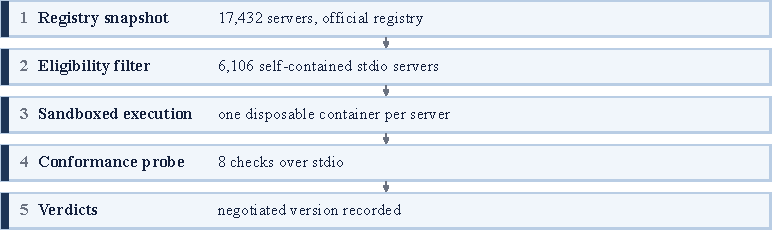
\includegraphics[width=\linewidth]{figures/pipeline.pdf}
  \caption{Measurement pipeline. Every eligible server is installed and executed in
  its own disposable container, then driven through the conformance probe. The protocol version each server
  negotiates is recorded with its verdicts, and no check depends on it.}
  \label{fig:pipeline}
\end{figure}

\subsection{Sampling frame}\label{sec:frame}
We crawl the official MCP registry (\texttt{registry.modelcontextprotocol.io})
via its cursor-paginated API, retaining the latest published version of each
server, which yields \Nframe{} unique servers. Each server declares zero or more
\emph{packages} (installable artifacts on npm, PyPI, OCI, NuGet, or Cargo) and/or
\emph{remotes} (hosted HTTP endpoints). Our study population is the set of servers
that are (i) locally installable, (ii) use the \texttt{stdio} transport, (iii)
distributed on npm or PyPI (the two dominant registries), and (iv)
\emph{self-contained}: they declare no required environment variable or argument
that lacks a default. Criterion (iv) restricts us to servers that a client could
launch without provisioning secrets, which limits what mass execution can do to
third-party systems and keeps the population reproducible.

Applied in order, the criteria remove \NFunnelInactive{} entries whose registry status
is not active, \NFunnelRemote{} that declare no package and are reachable only as a
hosted endpoint, \NFunnelNoStdio{} whose packages use another transport,
\NFunnelOtherReg{} whose stdio packages are published outside npm and PyPI (OCI images,
NuGet, MCP bundles), \NFunnelEnv{} that require an environment variable with no default,
and \NFunnelArg{} that require a launch argument with no default. \NFunnelEligible{}
servers remain. The frame is the denominator for every rate, and we launch all of it,
which makes the measurement a census of the eligible population rather than a sample.

We validated the filter in two ways. A second implementation, written from the four
criteria as stated here and sharing no code with the harness, reaches the same
decision on all \Nframe{} registry entries. A stratified sample of entries from each
exclusion class and from the eligible set, with the fields each decision rests on, was
read against the registry record, and each decision follows from its fields. The
script and the sample are released.

\subsection{Conformance harness}
The harness, \texttt{mcpprobe}, is a minimal, hand-written JSON-RPC
client speaking line-delimited messages over the server's stdio. We do not
use an official SDK client. To observe raw behavior, including responses to
malformed frames, the probe must not inherit any SDK-side correction or
validation. The harness offers protocol version \texttt{2025-06-18} at
initialization (the then-current revision was \texttt{2025-11-25}), records the
version the server \emph{negotiates}, and records it with every result. A server that
supports the offered version must answer with it, and \NVerOffered{} of
\Nresponders{} responders did. The rest negotiated three other revisions:
\NVerDowngraded{} settled on an older one, the oldest dating to 2024-11-05, and
\NVerAhead{} answered with a revision newer than the one offered, which the
lifecycle does not permit. Our checks encode requirements that every one of these
revisions states in the same terms, so no verdict depends on the negotiated version.
A requirement that moved between revisions would need a version-dependent rule, and
we add none.

Each server is driven through the following checks, whose identifiers align with
the categories of the official \texttt{modelcontextprotocol/conformance} suite
where an analogue exists:

\begin{itemize}
  \item \textbf{server-initialize}: the \texttt{initialize} request must return a
    result carrying a protocol version and a capabilities object, after which the
    harness sends \texttt{notifications/initialized}.
  \item \textbf{ping}: a \texttt{ping} must return an empty-object result.
  \item \textbf{tools-list}: if the server advertises the tools capability,
    \texttt{tools/list} must return an array in which every entry has a
    \texttt{name} and an \texttt{inputSchema} object.
  \item \textbf{tools-schema-valid}: each declared \texttt{inputSchema} must be a
    valid JSON Schema (checked by meta-validation).
  \item \textbf{tools-call-unknown}: calling a non-existent tool must be rejected.
    The specification's Error Handling section categorizes ``Unknown tools'' under
    \emph{Protocol Errors} (standard JSON-RPC errors) and illustrates this with a
    \texttt{-32602} example, as opposed to \emph{Tool Execution Errors} reported as
    a result with \texttt{isError: true}. This categorization is prose plus an
    example, and it uses no RFC-2119 \textsf{MUST}/\textsf{SHOULD} keyword. A
    diverging response is never scored as a ``violation''. Each server's choice
    between the two mechanisms is recorded (see \textsf{error-as-result} below).
  \item \textbf{tools-call-invalid-args}: for a tool with a typed required
    property, calling it with a wrong-typed value should be rejected. The spec is
    ambiguous here, since it lists ``Invalid arguments'' under Protocol Errors
    but ``Invalid input data'' under Tool Execution Errors. We count \emph{either} a
    protocol error \emph{or} an \texttt{isError} result as acceptable, and flag only
    a plain success response (the tool ran on ill-typed input) as a defect.
  \item \textbf{malformed-json}: after receiving a syntactically invalid frame, the
    server must not crash or hang, and a subsequent \texttt{ping} must still succeed.
  \item \textbf{stdout-purity}: under the stdio transport, the server must emit only
    protocol messages on stdout, and any non-JSON line is a channel-corruption defect.
\end{itemize}

\subsection{Grading and the error-as-result category}
Verdicts are \textsf{pass}, \textsf{fail}, \textsf{warn}, \textsf{skip}, and one
category introduced by calibration: \textsf{error-as-result}. When validating the
harness against the official reference servers (\texttt{server-memory},
\texttt{server-everything}), we found they answer an unknown-tool call not with the
specified JSON-RPC \texttt{-32602} error but with a \emph{successful} response whose
\texttt{result.isError} flag is set. Because this behavior originates in the
official SDKs, it reaches most of the ecosystem, and it earns its own verdict
category. Its prevalence is a result in its own right.

\subsection{Sandbox}
Each server runs in a fresh container (\texttt{node:22-slim} for npm, an \texttt{astral-sh/uv} image for
PyPI) with a memory cap, a single CPU, a PID limit, \texttt{no-new-privileges}, all
Linux capabilities dropped, and no host filesystem mounts. The harness supports two
probe conditions. In the \textbf{two-phase}
condition, an online install pass populates the cache and the conformance probe then
runs with \texttt{-{}-network=none}, so no server code has network access while it is
being measured. In the \textbf{single-phase} condition the network is available
throughout, and install and probe occur together in one ephemeral container. The
census reported here was measured in the single-phase condition, for the operational
reasons given in Section~\ref{sec:method-env}, and Section~\ref{sec:threats} carries
the consequences for validity.

\subsection{Execution environment and probe condition}
\label{sec:method-env}
The census was executed on a single disposable cloud instance (no cloud credentials attached) using the online single-phase condition: install and probe occur
in one ephemeral \texttt{-{}-rm} container per server, with nothing cached between
servers, which keeps disk usage bounded across the full ecosystem. The recorded
launch command of every run confirms that no volume was mounted. We did not run a
controlled comparison of the two conditions. In development runs on smaller subsets
we saw the same error-as-result prevalence and the same silent type non-enforcement
among responding servers under both. Handshake yields from those runs are not
comparable, because the subsets differed.

Two groups of runs ended for reasons outside the server's control. \NKilled{}
probes (\NKilledPct{}) were killed with exit 137 by either the memory cap or an
automated guard that reclaims host disk space, and the census does not record which.
Another \NHarnessError{} (\NHarnessErrorPct{}) aborted on a harness-side error before
any check ran. Only one of these \NInterrupted{} runs had completed a handshake
first, and the rest can only lower the reported yield.

\subsection{SDK-level confirmation}
\label{sec:sdk-probe}
Where a conformance failure concentrates in one SDK family, the census cannot
say whether the library permits the failure or the authors introduced it
independently. For the input-validation result we probed the SDK on its own. We build
two minimal servers, each exposing one tool that declares a single required string
property. One uses the low-level \texttt{Server} API and the other the high-level
\texttt{McpServer} API, both on the same SDK release. Each is driven with the harness
check used in the census: a \texttt{tools/call} carrying an
integer where the declared schema requires a string. The construction is otherwise
identical, so any difference in outcome is a property of the API path. We report the
result in Section~\ref{sec:consequences}, and the two servers and the probe script
are released with the harness.

\subsection{Funnel accounting}
RQ1 asks whether a server runs, and we count every stage:
declared $\rightarrow$ eligible (self-contained stdio npm/PyPI) $\rightarrow$
container started $\rightarrow$ process launched
$\rightarrow$ handshake completed $\rightarrow$ probed. Servers that never complete a
handshake are classified into startup-failure categories
(Section~\ref{sec:results}) from their exit code and stderr, which accounts for the
lost yield.
Runs broken by the harness are a separate outcome, reported with the funnel and
excluded from the graded population, because they measure our instrument.


\section{Results}
\label{sec:results}

We launched all \Nattempted{} servers in the eligible frame, and on \NHarnessError{}
of them our own probe failed on a broken pipe or an uncaught exception, leaving those
runs with no verdict about the server. We report them with the funnel and exclude them
from every denominator, which leaves \Nprobed{} graded servers.

\subsection{RQ1: Runnability and the startup funnel}
Once the entry-point artifact described in Section~\ref{sec:rq5} is corrected,
\HandshakeCountCorr{} of \Nprobed{} servers complete the MCP handshake, a rate of
\HandshakeRateCorr{}, against an uncorrected census figure of \HandshakeRateCl{}. Both
are lower bounds, because the census did not pass the launch arguments some registry
entries declare (Section~\ref{sec:threats}). Roughly two in
five never serve the protocol, and Figure~\ref{fig:failures} classifies those
failures by cause.

Servers that only need credentials or configuration are counted apart from servers
that crash, since a missing setting is a documentation gap. Most failures happen
\emph{after} a successful install: the package downloads, then the process crashes,
hangs, or exits without speaking the protocol. The software fails after the packaging
has done its job. A concurrent random draw of 400 npm
servers reports a 48.8\% handshake rate~\cite{randomdraw2026}, against \NpmRate{} for
the npm servers in our census. That study argues that curated frames select for
servers that work, and reports 66.7\% for a hand-curated frame under its own
instrument, which is close to our figure. Our frame is not curated: it is every
eligible server in the snapshot, with no popularity filter and no repair of a server
that fails to start. The difference we can name is the snapshot. Theirs is drawn from
a registry of 24,135 servers against the \Nframe{} in ours, and a registry that grew
from 3,510 to 18,966 servers in 88.6 days~\cite{registrydrift} is mostly newer
entries by the later date. Whether a newer cohort starts less often is a question a
single snapshot cannot settle.

\begin{figure}[t]
  \centering
  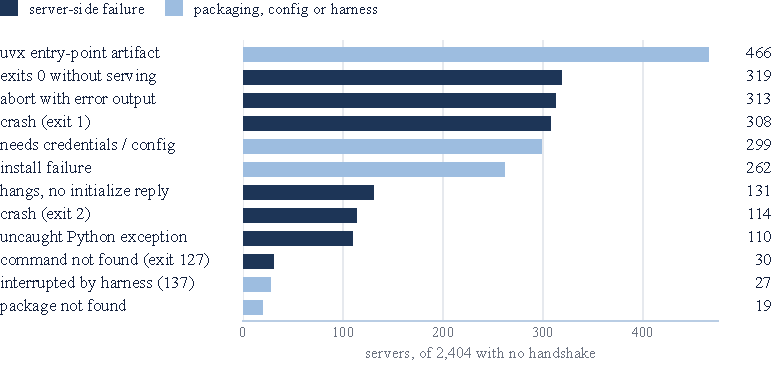
\includegraphics[width=\linewidth]{figures/failures.pdf}
  \caption{Why servers never reach a handshake. Configuration requirements and the
  entry-point artifact are separated from true startup failures.}
  \label{fig:failures}
\end{figure}

\input{tables/startup}

\subsection{RQ2--RQ3: Conformance and robustness}
Table~\ref{tab:verdicts} reports the verdict distribution for each check over the
\Nresponders{} responding servers, with 95\% Wilson confidence intervals. Lifecycle
and tool-listing conformance are high, and the discriminating checks are error handling,
argument type enforcement, and malformed-input survival. \NoTypecheckRateCl{} of
responders failed to reject a wrong-typed required argument, which
Section~\ref{sec:consequences} decomposes into the servers that reported the problem
anyway and the smaller class that did not. \MalformedDiesRateCl{} failed to recover from a
malformed frame, which we classify as a robustness and conformance failure. The
security reading does not survive the transport: under stdio the client is the parent
process and the sole writer to the server's standard input, and a party able to
deliver a malformed frame can already terminate the subprocess. JSON-RPC 2.0, on which MCP is built,
nonetheless defines a parse-error response for this case and requires a reply to
every subsequent request~\cite{jsonrpc}, and these servers give neither. One
maintainer who reproduced the finding made this argument, and the classification here
follows it (Section~\ref{sec:threats}).

\input{tables/verdicts}

\subsection{RQ3 refined: what a failure to reject returns to the client}
\label{sec:consequences}
The \texttt{tools-call-invalid-args} verdict records whether a server rejects an
argument that violates its own declared schema. As a protocol judgment that
is correct, but it cannot tell a client what it received, because two different
behaviors produce the same verdict. A server may validate the input and
report the problem in the result \emph{text} without setting \texttt{isError}, which
is non-conformant but leaves the information available. Or it may execute the tool
and return ordinary-looking output, which does not. We separate the two by
classifying the recorded response of every server in this category
(Figure~\ref{fig:consequences}, Table~\ref{tab:consequences}).

\begin{figure}[t]
  \centering
  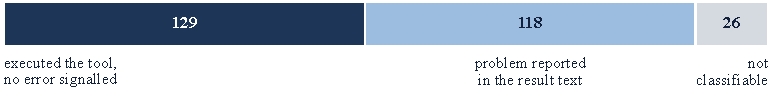
\includegraphics[width=\linewidth]{figures/consequences.pdf}
  \caption{The coarse verdict splits in half. Only the left segment is undetectable
  by the client: the tool ran on input its schema rejects and returned a well-formed
  result carrying no error indication.}
  \label{fig:consequences}
\end{figure}

Of \NAcceptInvalid{} such servers, \NInBandError{} (\InBandShare{}) reported the
problem in the result text. The server noticed, and a client willing to parse prose
could too. \NSilentExec{} (\SilentExecShare{}) executed the tool and returned a
result with no indication that anything was wrong. For \NUnclassifiable{} the
response could not be classified from the transcript. The hazard class is
\SilentExecRateCl{} of responding servers, smaller than the \NoTypecheckRateCl{} of the
raw verdict, and we report the smaller figure.

Splitting the two takes a classifier, and ours is a keyword rule over an English
error vocabulary. To measure what it gets wrong, a human rater labeled a stratified
sample of \ValN{} responses against a codebook fixed before any item was read, with
the classifier's answer hidden. The two agreed on \ValAgree{} of \ValN{}
(Cohen's \(\kappa = \ValKappa{}\)).

The errors are asymmetric. Of the responses the classifier calls silent execution,
the rater agreed on \ValSilExecPct{} (\ValSilN{} items), giving a precision of
\ValPrecision{}. Of those it files as reporting the problem in prose, the rater found
\ValInbExecPct{} were tools that had run anyway (\ValInbN{} items), giving a recall of
\ValRecall{}. Reweighting each stratum by its size in the census puts the true count
near \NSilentExecCorrected{} rather than \NSilentExec{}, in a range of
\NSilentExecCorrectedLo{} to \NSilentExecCorrectedHi{}. The keyword rule
under-counts, and \NSilentExec{} is the conservative figure. We report it as the
headline and treat the corrected range as the better estimate of the true rate.

The
specification's security requirements state that servers \textbf{MUST} validate all
tool inputs~\cite{mcpspec}. A server that executes a tool on an argument contradicting
its own published schema has not validated that input. These \NSilentExec{} servers
fail an explicit RFC-2119 requirement, as do the servers that write non-protocol
output to stdout, which the stdio transport forbids with a \textsf{MUST NOT}.

Here SDK attribution narrows the cause further than it does for the
error-reporting divergence. \SilentExecTS{} of the \NSilentExec{} are built on
the official TypeScript SDK and \SilentExecPy{} on either Python SDK, against
responding populations of \SDKPopTS{} and \SDKPopPy{} respectively. A behavior absent
from one language ecosystem and concentrated in another points to the library, and we
went on to test the SDKs (Section~\ref{sec:sdk-probe}). We ran this on
\texttt{@modelcontextprotocol/sdk} 1.30.0 and again on 1.30.1, the current release on
27 September 2026. On both, a server built with the low-level \texttt{Server} API publishes an
\texttt{inputSchema} in \texttt{tools/list} and the SDK then does not check
\texttt{tools/call} arguments against it. A tool declaring a string property, called
with an integer, runs and returns a well-formed result. The same tool built with the
high-level \texttt{McpServer} API, whose schemas carry type information the SDK
already validates, rejects the identical call with an \texttt{isError} result. We did
not test the Python SDKs under the same conditions, and their absence from this
population stands as an observation only. Within
the TypeScript SDK the gap is that one supported construction path publishes a
contract the library never enforces. The servers on that path have not declined a check
the SDK offered them. Of the \SilentExecTS{} TypeScript-SDK servers,
\SilentExecTSCaret{} declare a caret range and none declares an exact version.
Because each server was installed fresh, those ranges resolve to the newest 1.x. The
behavior is current, and a fix on the 1.x line would reach almost all of these
servers at their next install.

The unknown-tool divergence has a merged fix that deployed servers do not show. The
SDK's tracker records tool resolution as corrected in March 2026, four months before
our crawl. The change moves the tool-not-found check outside the handler's
\texttt{try} block, letting it propagate as a protocol error~\cite{sdkpr1389,sdkissue1510}.
We rebuilt the minimal high-level server on releases 1.28.0, 1.29.0 and 1.30.1 and
sent the same unknown-tool call. All three answer with an \texttt{isError} result
whose text reads \texttt{MCP error -32602: Tool \ldots{} not found}. The protocol
error is raised and then delivered inside a successful response, where a client
branching on JSON-RPC errors cannot see it. This explains a puzzle in our own data:
the census ran after the fix shipped, and the rate did not move.

The low-level path loses the tool name as well, which we had not tested. That API
takes one handler for every \texttt{tools/call} request, and the handler receives the
requested name without the library checking it against the declared tool list. Our
probe asked a low-level server for a tool it does not have and received that server's
ordinary answer, reporting a clean scan of code it was never given. Nothing in the
response marks the tool as missing.

Table~\ref{tab:consequences} shows what came back. The clearest cases are those
where the argument cannot be turned into what the schema asked for. A Hacker News tool
asked for top stories with a limit of \texttt{"not-a-number"} returned an empty feed,
which an agent reads as there being no stories. A regulatory tool asked for deadlines
within \texttt{"not-a-number"} days returned a dated snapshot, and a trading tool
returned a report whose requested and returned counts are both null. In the other
cases an integer was sent where a string was declared, and a runtime that stringifies
it may answer correctly: a code scanner handed \texttt{12345} reported no imports in
it. Every reply is a well-formed success. At the protocol level none can be told apart
from a correct answer, since there is no error code and no \texttt{isError} flag, and
each server published a schema that would have caught the call and then left it
unenforced.

\input{tables/consequences}

\subsection{RQ4: Where practice and specification disagree, and which one moved}
\ErrAsResultRateCl{} of responding servers answered a call to a tool that does not exist
with an \texttt{isError} tool-execution result instead of a JSON-RPC protocol error. The
specification's error-handling section lists ``unknown tool'' under \emph{Protocol
Errors} and illustrates it with a \texttt{-32602} example~\cite{mcpspec}, and attaches
no RFC-2119 keyword. The harness logs which mechanism each server uses, and neither
is scored as a violation (Section~\ref{sec:threats}).

The specification has been moving toward what servers do. SEP-1303, now
accepted and reflected in the specification, reclassified input validation errors from
protocol errors to tool execution errors on the grounds that a model can only
self-correct from an error it can see~\cite{sep1303}. SEP-2145, open at the time of
writing, proposes the same move for tool resolution failures, covering unknown and
disabled tools. Its stated rationale is that the change ``aligns specification with existing
Python and TypeScript SDK behavior''~\cite{sep2145}. We can say how much of
the deployed ecosystem that alignment already describes: \ErrAsResultRateCl{} of
responding servers. (Aggregate figures from this census were posted to the
proposal's discussion thread while it was open.) The other \NotErrAsResultPct{} do
not form one population: \UnknownProtoErrCount{} servers emit a protocol error coded
\texttt{-32602} or \texttt{-32601}, \UnknownWrongCodeCount{} use some other code, and
\UnknownProseCount{} return a plain success that states the failure only in its text,
a mechanism neither proposal describes.

To explain the uniformity, we attribute each server to its SDK from its resolved
dependency graph (Figure~\ref{fig:sdk}, Table~\ref{tab:sdk}). We take the exact
package version the probe launched and resolve its runtime dependencies through
deps.dev. A server that reaches an SDK through a third-party wrapper is credited
to that SDK and not to the residual. \SDKDirect{} servers name an SDK among their own
dependencies, and \SDKIndirect{} reach one only through a wrapper. For
\SDKUnattributed{} we have no graph: the package or the probed version has since been
withdrawn from its registry. The behavior tracks the SDK: the
official TypeScript and Python SDKs and the FastMCP framework all default to it. A
small number of TypeScript-SDK servers emit the protocol error, which shows the
alternative is reachable within the SDK without being its default, and the official
reference servers behave the same way.

Our attribution recognizes a fixed list of known SDK package names, and the residual
\textsf{no-known-SDK} category holds servers with none of those names anywhere in
their runtime graph. Such a server may still have vendored an SDK at build time.
Resolving the graph transitively moves servers that inherit an SDK through a wrapper
into that SDK's family. That leaves the residual as the sharpest contrast in the
table: \SDKNoSDKRate{} of its \SDKNoSDK{} servers answer an unknown tool with an
\texttt{isError} result, against about nine in ten in every official-SDK family.
A few SDK defaults, whether used first-hand or through wrappers, account for this
behavior across the ecosystem, and where no known SDK is present it falls to about
half. The residual is not free of SDKs, only of SDKs our attribution can see, and
the next paragraph shows what one of them does.

\paragraph{A third SDK, found inside the residual}
A maintainer's report gave us a way to test that claim on a library we never sampled
as a family. Their server failed our malformed-frame check and contains no framing
code at all: it is built on the official Go SDK, whose stdio transport ends the
session on a decode error (Section~\ref{sec:threats}). Our attribution had recorded it
as having no known SDK, because a Go binary published through npm declares no MCP
dependency. Reading each residual server's repository language finds
\NGoResidual{} such Go servers, all of which complete a handshake.

They behave as a family, and not as the rest of the population does. \NGoMalformedFail{}
of the \NGoResponding{} fail the malformed-frame check, a rate of \GoMalformedRate{}
against \MalformedDiesRateCl{} across all responders. On the unknown-tool check every
one of the \NGoResponding{} returns the JSON-RPC protocol error, where
\ErrAsResultRateCl{} of responders return \texttt{isError}. Under the population rate
for that response, eleven consecutive protocol errors would arise by chance with
probability below \(10^{-15}\).

Two independent checks, opposite defaults, one library. This is the same claim the
error-as-result result makes, tested on a library that reached our census only as a
compiled binary, and it is the cleanest evidence we have that these verdicts record
an SDK rather than an author. The set is small and was identified by repository
language rather than by dependency graph, so we report it as a confirmation of the
mechanism and not as a rate for the Go ecosystem.

\begin{figure}[t]
  \centering
  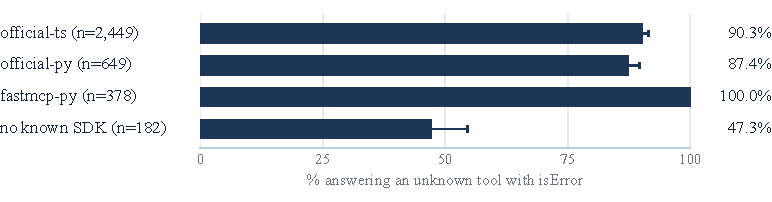
\includegraphics[width=\linewidth]{figures/sdk.pdf}
  \caption{Unknown-tool responses by SDK family. In every family, most servers answer with an \texttt{isError} result. Bars show 95\% Wilson intervals, and families
  with fewer than 25 servers appear in Table~\ref{tab:sdk} only.}
  \label{fig:sdk}
\end{figure}

\input{tables/sdk}

\subsection{RQ5: Correlates}
\label{sec:rq5}
We test whether runnability and conformance correlate with the package registry
(Figure~\ref{fig:byregistry}). Runnability differs: npm servers complete a
handshake much more often than PyPI servers (\NpmRate{} of \NpmN{} against
\PypiRateRaw{} of \PypiN{}, a difference of \GapRunnableCl{}). Conformance does not:
the same publisher-cluster bootstrap puts the error-as-result difference at
\GapErrAsResultCl{}, an interval spanning zero. Both comparisons use the same method,
and neither rests on a stronger footing than the other. The pattern follows from RQ4,
where the divergence is inherited from the SDKs and both language ecosystems' SDKs
share the same default. The registry a server ships on changes whether it
starts but not whether it conforms.

Part of this gap came from our own launcher, and we corrected for it. We launch PyPI
servers as \texttt{uvx <package>}, which resolves only
if the package's console script is named after the package. npm's \texttt{npx}
resolves the entry point from \texttt{package.json} and has no such requirement.
\NEntrypointBlocked{} PyPI servers (\EntrypointBlockedPct{} of the PyPI population)
installed successfully but were never launched for that reason and no other. Our
classifier identifies \NEntrypointSeen{} such rows in the census, the completed
re-probe covers \NEntrypointBlocked{} of them, and \NEntrypointUnreprobed{} were
missed. We re-probed those servers with the entry point resolved from the installed
package metadata. \EntrypointRecovered{} (\EntrypointRecoveryRate{}) then completed a
handshake, and the rest failed for reasons unrelated to naming (Python exceptions,
hangs, undeclared configuration). Correcting for this raises PyPI runnability from
\PypiRateRaw{} to \PypiRateCorr{} and the overall census figure to
\HandshakeRateCorr{}, which we report as the headline throughout. The npm--PyPI gap
narrows from \GapRaw{} to \GapCorr{} percentage points but stays large.

The entry-point problem is also a finding about the ecosystem. Registry metadata does
not record a server's entry point, and a client working from the registry and nothing
else cannot launch a fifth of published PyPI servers. Once the entry point is
resolved, nine in ten of those servers still fail to start, and a listing in the
registry says nothing about either outcome.

\begin{figure}[t]
  \centering
  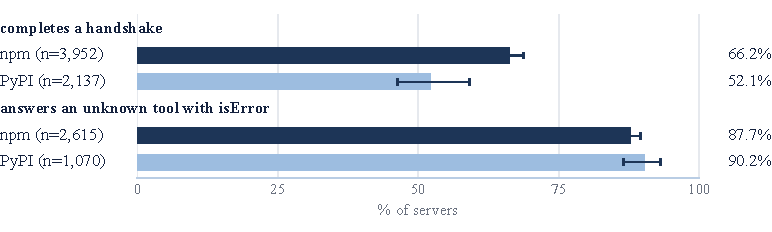
\includegraphics[width=\linewidth]{figures/by_registry.pdf}
  \caption{Handshake yield (PyPI after the entry-point correction) and the
  error-as-result rate for unknown tools, by package registry, with 95\% intervals
  from a publisher-cluster bootstrap.}
  \label{fig:byregistry}
\end{figure}


\section{The Same Frame, Sixty-Nine Days Later}\label{sec:rerun-top}
\label{sec:rerun}

The census frame is fixed at the snapshot of 19 July 2026, so re-running it probes
the same servers, at the same declared versions, with the same launch commands. What
those commands resolve is not fixed. Each launch installs the package and whatever
its dependency ranges admit on the day. We re-ran the complete frame on \SeptDate{},
sixty-nine days later, with the harness unchanged.

\paragraph{What the re-run found}
\NSeptHandshake{} of \NSeptGraded{} graded servers complete a handshake,
\SeptHandshakeRate{} against \HandshakeRatePoint{} in July. \NLost{} servers that
answered in July no longer answer, and \NGained{} that did not answer now do.

Conformance did not change. On the \NPaired{} servers that answered in both runs,
error-as-result was \PairedEarBefore{} in July and \PairedEarAfter{} in September, silent
type non-enforcement \PairedTypeBefore{} and \PairedTypeAfter{}, and failure to recover
from a malformed frame \PairedMalBefore{} and \PairedMalAfter{}. Rates computed over each
run's own responders move slightly more, type non-enforcement from
\NoTypecheckRateCl{} to \SeptNoTypecheck{}, but that is a change in who answers rather
than in how they answer: the servers September lost had a type non-enforcement rate of
\LostTypeRate{} in July, so removing them raises the rate among those that remain. The
instrument reports the same behavior from the same servers. What changed is how many of
them start.

\paragraph{One dependency release accounts for most of the loss}
Of the \NLost{} servers that stopped answering, \NLostUnchanged{} were probed at the
same declared version with the same launch command as in July, so the servers
themselves did not change. \NSDKTwoBroke{} of them fail with one of two signatures in
their own output: the official Python SDK's compatibility message, which states that
this is \texttt{mcp} 2.x and that \texttt{FastMCP} has been renamed to
\texttt{MCPServer}, or an \texttt{AttributeError} for a handler-registration
decorator that the same major version removed from the low-level
\texttt{Server} class.

That SDK published 2.0.0 on \SDKTwoDate{}, nine days after our snapshot.
\NSDKTwoRange{} of the \NSDKTwoBroke{} declare the dependency as a floor or a range
rather than an exact pin, so the same launch command resolved 1.x in July and 2.x in
September.

Three observations separate this from a fault in our own instrument or host.
The effect is confined to one package ecosystem: \NpmLost{} of \NpmWas{} npm servers
that answered in July stopped answering (\NpmLostRate{}), against \PypiLost{} of
\PypiWas{} on PyPI (\PypiLostRate{}). A host, network or harness fault would not
respect that boundary. The attribution comes from the servers' own stderr rather than
from our classification. And the failure is reversible: we re-launched a random
\NPinTested{} of the affected servers with the SDK constrained below 2.0 and
otherwise unaltered, and \NPinRestored{} completed a handshake.

Restricting attention to the servers this could affect, \NPySDKWas{} PyPI servers
attributed to a Python MCP SDK completed a handshake in July and \NPySDKNow{} do now.
\PySDKLostCI{} of them stopped working, and no author changed anything.

\paragraph{What this run is and is not}
It is not an independent census. It is the same frame re-probed, so it says nothing
about servers published after July, and the \NGained{} recoveries are not a sample of
anything. The July run remains the measurement this paper reports, because its
conformance verdicts were collected when the population was largest. The re-run's
contribution is the comparison.


\section{Discussion}\label{sec:discussion}
\paragraph{The specification and the SDKs}
SEP-2145 is close to settled before anyone votes on it. SEP-1303 already
reclassified input validation failures as tool execution errors, arguing that a model
can only correct an error it sees~\cite{sep1303}, and SEP-2145 proposes the same for
unknown tools~\cite{sep2145}. Adopting it would not change how servers behave. It
would change the document to describe what \ErrAsResultRate{} of responding servers
already do. Rejecting it would make \ErrAsResultCount{} servers wrong
overnight, and nobody is going to fix them. Nor is there a coherent minority to
protect: of the servers that do not answer with \texttt{isError},
\UnknownProtoErrCount{} emit the protocol error the specification illustrates,
\UnknownWrongCodeCount{} emit a different code, and \UnknownProseCount{} report the
failure only in prose.

The second point matters more than the first. This behavior was not chosen. Server
authors did not weigh the two mechanisms and pick one; they inherited a default that
is the same across the official TypeScript and Python SDKs and the third-party
wrappers built on them. So \ErrAsResultRate{} is not a vote, and it should not be
read as community consensus about the right design. It is a count of who used an SDK.
The same fact cuts the other way, and more usefully: one change at the library layer
moves thousands of servers at once, in whichever direction the specification chooses.
The limit of that lever is visible here too. The unknown-tool fix recorded on the
TypeScript SDK's tracker in March 2026 shipped four months before our census, and the
rate did not move.

\paragraph{Silent execution is a different kind of finding}
The unknown-tool divergence is a disagreement about which channel carries an error.
Either way the client is told that something failed. Silent execution tells the
client nothing failed. The specification obliges every server to validate the inputs
it is given, no pending proposal would relax that obligation, and so there is no
argument that the specification will catch up.

A client that receives one of these answers cannot tell it from a correct one. There
is no error code, no \texttt{isError}, nothing to branch on. A tool that scans code
for package imports, handed the integer \texttt{12345}, replied \texttt{CLEAN}, which
is what a real clean scan looks like. The agent cannot retry, cannot repair the
argument, and cannot warn the user. It carries the wrong result forward. And
\NSilentExec{} is a lower bound, because we credited any error-like wording in a reply
as a report. This is also not \NSilentExec{} careless authors. \SilentExecTS{} of them
are built on the official TypeScript SDK, whose low-level \texttt{Server} API
publishes a tool's \texttt{inputSchema} and then never checks an incoming call against
it (Section~\ref{sec:consequences}). The default does the publishing and leaves out
the checking.

\paragraph{Startup failure and what a registry could do about it}
Two in five installable servers never serve the protocol, and nothing in a registry
listing says so. A registry could try a handshake once before listing an entry and
show the outcome. It need not delist anything; it need only tell people. The check is
cheap, and we ran it across the whole ecosystem.

Two further gaps in the registry record are ours to report because we hit them. The
registry does not record an entry point, which left \NEntrypointBlocked{} PyPI servers
impossible to launch from registry data alone, and cost our own measurement about two
percentage points of apparent PyPI yield until we corrected for it
(\PypiRateRaw{} uncorrected against \PypiRateCorr{} after). And required configuration is not recorded either: \NNeedsConfig{}
servers failed for no reason other than a setting that nothing told us to supply.
Neither is a defect in the server. Both are things a client cannot learn without
running the software.

\paragraph{What running the servers shows that reading them cannot}
None of the above is visible to a study that reads code or metadata. The static
ecosystem studies~\cite{mcpfirstglance,mcplandscape} cannot see a server that does not
start, and they cannot see one that answers a poisoned call as though it were
ordinary. The artifact's presence in a registry says almost nothing about the
artifact. The same lesson is reported for Jupyter notebooks, where publishing one and
running it turned out to be different
questions~\cite{notebookreproducibility}, and for Docker Hub images that share a
name~\cite{dockerhubimages}. It is also a caution about registries as a research
source~\cite{huggingfacehub}: our own entry-point problem was exactly that, a
launcher reading registry fields and getting them wrong.

One contrast in our data sharpens the point. Runnability differs sharply between the
two package registries, \NpmRate{} against \PypiRateCorr{}, while conformance among
the servers that do run does not. Packaging problems are per-ecosystem and
per-package. Protocol behavior is per-SDK. Fixing conformance means changing a few
libraries. Fixing runnability means changing thousands of packages. Those are very
different amounts of work, and only the first has a lever short enough to pull.

\paragraph{A moving specification}
The lifecycle we measure is being retired. Revision 2026-07-28 drops the
initialization handshake and negotiates a version on every request instead, with an
optional \texttt{server/discover} call for clients that want to ask up
front~\cite{mcpversioning}. Handshake-based behavior is now described as a backward
compatibility concern. Our population sits well behind that boundary:
\PctVerOffered{} of responders settled on 2025-06-18, and \NVerDowngraded{} answered
with something older still. This census records an installed base at the point its
mechanism left the specification, and measures the distance between the two. A server
published today inherits whichever default its SDK shipped with, and the revision that
removes the handshake reaches those servers only when their authors upgrade, which the
version spread here suggests is slow.

\paragraph{Recommendations}
For the specification: accept SEP-2145, state it with an RFC-2119 keyword rather than
an example, and add the unknown-tool case to the conformance suite so that it is
tested rather than described.

For SDK authors: validate \texttt{tools/call} arguments against the declared
\texttt{inputSchema} before dispatch, in the low-level \texttt{Server} API as well as
the high-level one, and check the tool name against the declared list. Most authors
never touch a default, so the default is the behavior.

For agent framework authors: do not treat the absence of \texttt{isError} as evidence
that a call succeeded. Validate arguments against the declared schema on the client
side, because \SilentExecRate{} of responding servers do not, and treat a server as
unproven until it completes a handshake.

For registry maintainers: run a handshake at publish time and show the result, and
record the entry point and the required configuration in the listing.


\section{Threats to Validity}
\label{sec:threats}

\paragraph{Construct validity}
Our verdicts operationalize ``conformance,'' and a poorly chosen operationalization
could over- or under-count. Our checks cover requirements that every revision in the
census states in the same terms, which keeps any server from being judged against a
rule that postdates the revision it negotiated, and we also distinguish normative
requirements from illustrative ones. The most prevalent divergence we report
(unknown-tool responses) is graded in its own \textsf{error-as-result} category and
never counted as a failure, because the specification expresses it only in prose and
an example, without an RFC-2119 keyword. We calibrated the harness on the
official reference servers before the study and confirmed it reproduces their
known-good behavior on every check except the SDK-level divergence we set out to
measure.

\paragraph{Internal validity}
The census ran in the single-phase condition, with the network available
during both install and probe (Section~\ref{sec:method-env}). This avoids penalizing
a server that legitimately contacts the network during initialization, but it does
not remove server-side outbound calls as a confounder. The exposure is concentrated
in one check: for \textsf{tools-call-invalid-args} we accept an \texttt{isError}
result as evidence that the server rejected the ill-typed argument. An
\texttt{isError} produced instead by an unrelated runtime or network failure is
indistinguishable to the harness, and would be counted as argument checking that did
not in fact occur. The rating pass below puts a number on that: a quarter of the
responses the classifier read as argument checking were, to a human reader, tools
that had run anyway.

A second artifact affects the same check. Where a tool declares several required
properties, the harness poisons one and fills the rest with placeholder values, so a
server may reject a placeholder and never examine the argument under test. We find
one such response in the \NAcceptInvalid{} we classified, which bounds the effect at
well under a percentage point, and a re-run records which property was poisoned so
the case can be excluded directly. The lifecycle, tool-listing, error-handling, malformed-input and
stdout-purity checks are local protocol behaviors and are not exposed to this
confound. A network-isolated replication would tighten the argument-checking result,
and the harness already supports that condition. Sandbox heterogeneity across
language runtimes is a further source of noise. We bound it by launching each package
at the version its registry entry declares and by recording every run's full launch
command, including the base-image tag.

\paragraph{External validity}
Our population is self-contained, locally-installable servers distributed on npm and
PyPI using the stdio transport. This excludes remote-only servers (which we cannot
execute without provisioning hosted infrastructure) and servers requiring
credentials (which we exclude for both ethics and reproducibility). We report the
size of each excluded class and confine all rates to the stated frame.
Whether remote and credentialed servers behave the same way is untested here. Agent
clients mostly launch local stdio servers, and we studied this population first.

\paragraph{Population counts and publisher clustering}
Because we census the eligible frame, the counts are population counts. The intervals
we report do not describe sampling error. They describe how far a rate would move if
the registry had drawn a different set of publishers, which is the uncertainty that
matters when a single publisher ships hundreds of servers from one template. The
\Nprobed{} servers in our frame come from only \Npublishers{} distinct registry
namespaces, and the distribution is heavy-tailed: the largest single publisher
accounts for \TopPublisherN{} servers (\TopPublisherPct{} of the census) and the ten
largest for \TopTenPct{}. Servers from one publisher frequently share a template and
behave near-identically; a binomial interval that treats them as independent trials
is therefore too narrow. Every interval in this paper comes from a bootstrap
over publishers rather than over servers. The widening is substantial: the handshake
interval is \HandshakeDesignEffect{} times wider than the binomial one
(\HandshakeRateCl{} against \HandshakeRate{}). Error-as-result becomes
\ErrAsResultRateCl{} and silent type non-enforcement \NoTypecheckRateCl{}. As a second
check we recompute each rate on a subset holding one server per namespace
(\NuniqPub{} servers): handshake yield \HandshakeRatePub{}, error-as-result
\ErrAsResultRatePub{}, silent type non-enforcement \NoTypecheckRatePub{}, and no
conclusion changes under either treatment. The largest publisher is atypical in
runnability at a \TopPublisherHandshake{} handshake yield, and its presence moves the
census figure by \TopPublisherDepressionPP{} percentage points.

\paragraph{Validating the response classifier}
The split between silent execution and an in-band report rests on a keyword rule, and
an unvalidated rule behind a headline number is exactly the weakness that recent work
found in MCP security scanners~\cite{mcpzoo}. We therefore fixed a codebook, drew a
stratified sample of \ValN{} responses, and had a human rater label each one with the
classifier's answer hidden. Agreement was \ValAgree{} of \ValN{}, Cohen's
\(\kappa = \ValKappa{}\). Precision is \ValPrecision{} and recall \ValRecall{}, so the
rule seldom invents a silent execution and regularly misses one. Reweighting by
stratum size puts the true count near \NSilentExecCorrected{}
(\NSilentExecCorrectedLo{} to \NSilentExecCorrectedHi{}) against the
\NSilentExec{} the rule finds, and we keep the smaller figure as the headline.

Two limits on that exercise. One rater labeled the sample, so the agreement measures
the rule against a single reader and not the reliability of two independent readers.
An earlier pass by the same rater, used for training and released alongside the
labels, is not part of this result: it was taken at speed and the tool revealed the
classifier's answer after each item, so those items were no longer blind. The sample
reported here is drawn from responses that rater had not seen.

\paragraph{Severity of the malformed-frame finding, and a limitation it exposed}
We initially characterized failure to recover from a malformed frame as a
denial-of-service primitive. A maintainer who reproduced the finding independently
argued that this overstates it, and the argument holds. Under the stdio transport
only the launching client writes to that standard input, and anyone able to
send it a malformed frame can already kill the subprocess. The specification also
places the obligation not to send invalid messages on the client. This paper
classifies the behavior as a robustness and conformance failure. The same maintainer
traced it in their own server to the official Go SDK's stdio transport. Like the
unknown-tool divergence, this check can measure an SDK default that the server only
inherits.
Another maintainer's fix exposed a limitation in our instrument. In their server the
process stayed alive while its parser absorbed the frames that followed, and the next
\texttt{ping} timed out. Our harness records a single verdict for
``did not answer after a malformed frame'' and does not distinguish a terminated
process from a desynchronized one. Both are conformance failures, but they are
different failures with different fixes, and \MalformedDiesRate{} aggregates
the two. Separating them requires per-server process-state tracking that the released
transcripts support but the current verdict does not encode.

\paragraph{Interrupted probes}
\(49\) probes (\(0.8\%\)) ended for reasons that may lie outside the server
(Section~\ref{sec:method-env}): \(32\) killed by the memory cap or the disk guard, and
\(17\) aborted by a harness-side error. Counting \(48\) of them as non-handshaking can
depress the handshake yield by at most \(0.8\) percentage points and does not affect
conformance rates. Each is identifiable in the released census rows by its exit code
or its missing verdicts.

\paragraph{Reproducibility}
Every number in this paper is regenerated by the released analysis scripts from the
released census rows, and we have checked that the regenerated values match the ones
printed here. The registry snapshot, launch commands, and package versions are
recorded. Census rows do not record the harness commit, but the code that produced
them is tagged \texttt{census-v1}, and the probe logic there is unchanged from the
version that was calibrated.

The registry changes daily, and the object of study is the snapshot of
19 July 2026.
A longitudinal study of the same registry shows how fast it moves, growing from 3,510
to 18,966 servers over 88.6 days~\cite{registrydrift}.


\section{Ethics and Responsible Disclosure}\label{sec:ethics}
This study executes third-party code and probes servers for defects, and it follows
the norms of responsible measurement research.

\paragraph{Safe execution}
Every server runs inside an isolated container during both installation and probing,
with all Linux capabilities dropped, no new privileges, bounded memory, CPU and
process counts, and no host filesystem access. The census was executed in the
single-phase condition, where install and probe share one ephemeral container and the
network is available throughout. The install phase executes arbitrary
\texttt{postinstall} and build scripts, and it receives the same isolation as the
probe. Server code also had network access while being measured, and to limit the risk
every container is discarded after a single server, while the entire census ran on a
disposable cloud instance with no credentials attached. Untrusted code could reach no
further than one throwaway host. The harness also supports a network-isolated probe
phase (\texttt{-{}-network=none}), which we recommend for replications that do not
need install and probe in a single pass. We execute no server that declares a
requirement for credentials, both because it lies outside our frame and because doing
so could send real requests to third-party systems.

\paragraph{Observed side effects of networked measurement}
Because the census ran with the network available, we audited the captured output
for evidence that server code produced effects outside its container. At least \OutboundFailPct{} of servers attempted an
outbound connection that failed and logged an error. A successful connection leaves
no trace in the captured output, and this figure is a lower bound. Our redactor caught credential-shaped values in the output of
\NCredRedacted{} servers, and on reading each one, four were live: three printed
session tokens they had generated for local use, and one auto-provisioned an API key
and account against a third-party service. The fifth printed a configuration example
whose key was a placeholder. The provisioned key is the class our frame's exclusion of credential-requiring
servers was meant to prevent, and we have redacted every such value from the released
dataset and asked the service to revoke the provisioned key and delete the account.
Excluding servers that \emph{declare} required
credentials does not exclude servers that \emph{acquire} them unprompted, which makes
declaration-based eligibility filtering a weaker ethical guarantee than it
appears. A network-isolated probe phase should be the default for
measurement at this scale, and we recommend replications use the harness's
two-phase mode. We used the single-phase condition because it let one disposable host run the
whole ecosystem, and the side effects above are what it cost.

\paragraph{Responsible disclosure}
Some of our findings concern robustness. A server that stops serving after a
malformed frame can desynchronize or strand a connected client, and so can a server
that emits non-protocol bytes on its stdio channel. We report these
only in aggregate and through anonymized case studies, and we do not publish a
name-and-shame list of individual servers. Security-relevant findings are recorded
in a private disclosure log with maintainer contacts resolved from registry
repository metadata. We reported \NMalformedReported{} of the \NMalformedDies{} servers that stop serving
after a malformed frame to their maintainers through their issue trackers; the
remaining \NMalformedUnreachable{} list no repository we could reach. At the time of
writing \NMalformedFixed{} of those reports are closed as resolved, and
\NMalformedReleased{} of the projects have published a release since closing them. One
maintainer corrected our severity assessment, and the paper follows that correction
(Section~\ref{sec:threats}). We also reported the input-validation gap in the
TypeScript SDK's low-level \texttt{Server} API (Section~\ref{sec:consequences}) to
the SDK maintainers, who have labeled it for design work on both the 1.x and 2.x
lines. We did not open an issue against each of the \NSilentNotices{} servers that run a
tool on an argument their own schema rejects. The defect we identify there belongs to the library.
\SilentExecTS{} of them are built on the SDK whose low-level API publishes a schema it
does not enforce, and a per-server report would tell an author their code is at fault
where our own analysis says it is not.
Notices are drafted and released with the harness so that any maintainer can check
their own server, their identities are withheld from the dataset, and the report went to the SDK, which
can fix it. The
remaining findings concern unknown-tool handling and stdout contamination, and they
are of lower severity and appear only in aggregate.

The released dataset withholds the identities of all \NWithheld{} servers carrying a
security-relevant finding, replacing each name with a stable pseudonym so the rows
remain linkable across files. That set includes every server in the silent-execution
class. Naming a server beside a transcript of it answering a poisoned call is a
claim about its author's work. The empirical standard for secondary data asks that
the reputation of the subjects be respected in the reporting of a study as well as
in its conduct. The registry snapshot in the release carries the same pseudonyms, so the withheld
set cannot be recovered from the release by subtracting the servers the census names
from the servers the frame lists. The registry itself is public, and someone who
compared the release with an archived copy of it could still recover which servers
were withheld. The comparison cannot reveal which finding belongs to which server,
nor any transcript, and we withhold both. Identities are restored only
where a maintainer has fixed the defect or asked to be named.

\paragraph{Registry and maintainer impact}
Our crawl pages sequentially through the registry's public API and backs off on
errors. Our installs draw each package once per probe from its public registry
in the ordinary way. The released harness lets any author check their own server's
conformance before publishing.


\section{Conclusion}\label{sec:conclusion}
Earlier studies measured the MCP server ecosystem statically, or ran servers to look
for vulnerabilities. We installed every eligible server in the official registry,
launched each in a disposable sandbox, and tested whether it follows the protocol.

\HandshakeRateCorr{} complete a handshake. The rest never serve the protocol, for the
reasons broken down in Figure~\ref{fig:failures}. Of the servers that respond,
\ErrAsResultRateCl{} report an unknown tool in the same way, and the cause is the SDKs
they are built on as a direct dependency or through a third-party wrapper.
An open proposal would change the specification to match this behavior, and our
numbers show how much of the ecosystem it already describes. A smaller group,
\SilentExecRateCl{}, run a tool on input their own schema rejects and return an answer
with no sign that anything is wrong. One was asked to scan an integer for package
imports and reported it clean, and the specification makes input validation a
requirement these servers do not meet.

A static scan or a registry crawl shows none of this. The harness and the dataset are
public, and others can repeat the measurement, extend it to remote and credentialed
servers, or check their own servers before publishing. Because the error-reporting
and input-validation behavior comes from a few SDKs, it can be changed there.


\backmatter

\bmhead{Acknowledgements}
The author conceived the study, made its design and interpretive decisions, and directed the writing. Claude (Anthropic), a generative AI system, used as Claude Opus 5 and Claude Opus 5.5, wrote the measurement harness and the analysis code, assisted with literature search, running the census and the statistical analysis, and drafted and edited the text under that direction. The interpretation and recommendations in the Discussion were written from answers the author supplied and were approved by the author. Every reference and every claim attributed to a cited source was checked against that source, and every number is regenerated from the released data by the released scripts. No AI system is an author, and the author takes full responsibility for the content.

\section*{Statements and Declarations}

\bmhead{Funding}
No funding was received for conducting this study.

\bmhead{Competing interests}
The author declares no competing interests.

\bmhead{Ethics approval}
This study executes and measures publicly published software packages. It involves
no human subjects and required no ethics board approval. Section~\ref{sec:ethics} states the
measures taken to limit harm to the maintainers whose servers were executed and to
the third-party services some of them contacted.

\bmhead{Data and code availability}
The conformance harness is available at \ArtifactURL{} with the analysis pipeline
and the disclosure-filtered census dataset, and the code that produced the census
is tagged \texttt{census-v1}. The release contains one record per probed server, carrying every verdict behind every number in this paper, and the same for the September re-run. It also holds the raw JSON-RPC transcripts, the registry snapshot that defines the sampling frame, the classified responses to the invalid-argument check, the blinded rating labels with their codebook, the pinning experiment and the eligibility validation. Together they recompute the funnel and every reported rate, and a test suite that runs on every change checks the harness verdicts and the release itself. Two
filters are applied and documented with the data. The identities of \NWithheld{}
servers with security-relevant findings are withheld pending disclosure, as is one
server whose maintainer asked to be removed. These servers keep every measurement,
but we publish neither their names nor their transcripts, and credential material
that servers emitted at runtime is redacted. Neither filter alters any verdict or
count, and the paper's figures regenerate from the release unchanged. The release
is archived on Zenodo under the concept DOI
\href{https://doi.org/10.5281/zenodo.22981443}{\texttt{10.5281/zenodo.22981443}}, which
resolves to the current version; the version this paper reports is
\texttt{10.5281/zenodo.22991985}.

\bmhead{Author contribution}
The sole author conceived and designed the study, directed the construction of the
harness and the analysis pipeline, ran the census, carried out the rating pass,
handled the disclosure process, and made the interpretive decisions in the
manuscript. The use of a generative AI system is described in
Section~\ref{sec:genai} and under Acknowledgements.

\bibliography{../refs}

\end{document}
